\maketitle
\tableofcontents
\newpage

\section{Zielsetzung}
Ziel des Versuches ist es, gekoppelte Schwingkreise im Hinblick auf Energietausch
mittels Schwebung und auf ihre Fundamentalschwingungen zu untersuchen.
\section{Theorie}
Die in diesem Versuch gekoppelten Schaltkreise bestehen aus der Induktivität
$L$ und der Kapazität $C$. Die Kopplung besteht aus einem Kopplungskondensator
$C_{\symup{K}}$.
\begin{figure}
  \centering
  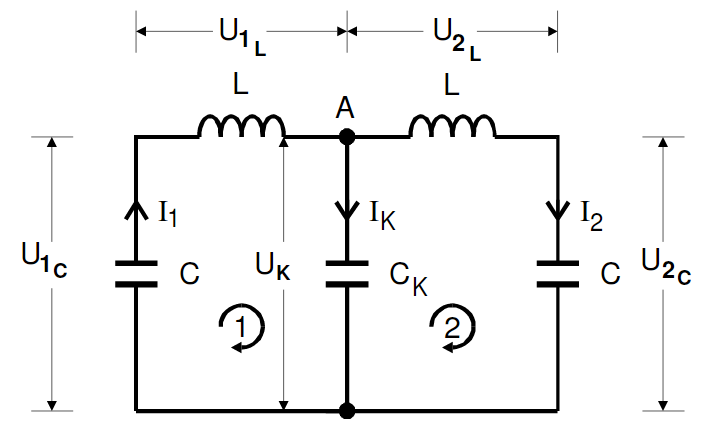
\includegraphics[scale=0.4]{theorie.png}
  \caption{Schaltbild zweier gekoppelter Schwingkreise \cite{anleitung}.}
  \label{fig:1}
\end{figure}
Aus Abbildung \ref{fig:1} lässt sich nun mithilfe der Kirchhoffschen Knoten-
und Maschenregel zwei Schwingungsgleichungen aufstellen
\begin{align}
    L\ddot{I}_1 + \frac{1}{C} \, I_1 + \frac{1}{C_{\symup{K}}} \left(I_1 - I_2\right) &= 0
    \label{eqn:1} \\
    L\ddot{I}_2 + \frac{1}{C} \, I_2 - \frac{1}{C_{\symup{K}}} \left(I_1 - I_2\right) &= 0 \, .
    \label{eqn:2}
\end{align}
Diese Differentialgleichungen sind voneinander abhängig und lassen sich deswegen
nicht ohne weiteres lösen. Durch Subtraktion von \eqref{eqn:1} und \eqref{eqn:2} erhält man
\begin{align}
    L \,  \frac{\symup d^2}{\symup d t^2} \left(I_1 + I_2 \right) + \frac{1}{C} \left(I_1 + I_2 \right) &= 0
    \label{eqn:3} \\
    L \,  \frac{\symup d^2}{\symup d t^2} \left(I_1 - I_2 \right) + \left(\frac{1}{C} + \frac{2}{C_{\symup{K}}} \right)
    \left(I_1 - I_2 \right) &= 0 \, .
    \label{eqn:4}
\end{align}
Damit lassen sich \eqref{eqn:3} und \eqref{eqn:4} unabhängig voneinander lösen; Die
Lösung von \eqref{eqn:3} ist hierbei eine harmonische Schwingung mit der Schwingungsfrequenz
\begin{equation}
    \nu_+ = \frac{1}{2\pi \sqrt{LC}} \, .
     \label{eqn:5}
\end{equation}
Diese Schwingung wird als gleichphasig bezeichnet. Diese wird dadurch ausgezeichnet,
dass beide Schwingkreise so schwingen, als wäre keine Kopplung vorhanden. Wenn man zwei
durch eine Feder gekoppelte Fadenpendel in die gleiche Richtung gleich weit auslenkt,
dann wird die Feder weder gestaucht noch gestreckt, sie verharrt in ihrem unausgelenktem
Zustand. Genauso verhält es sich mit zwei Schwingkreisen, die mit gleicher Amplitude und
Phase anfangen zu oszillieren.

Die Lösung von \eqref{eqn:4} hat die Schwingungsfrequenz
\begin{equation}
  \nu_- = \frac{1}{2\pi \sqrt{L \left(\frac{1}{C} + \frac{2}{C_{\symup{K}}} \right)^{-1}}} \, .
  \label{eqn:6}
\end{equation}
Diese Art der Schwingung wird als gegenphasig bezeichnet. Die Oszillation beginnt
mit gleicher Amplitude, aber entgegengesetzter Phase. Offensichtlich gilt
\begin{equation*}
    \nu_- > \nu_+ \, .
\end{equation*}
$\nu_+$ und $\nu_-$ sind die Frequenzen zu den Fundamentalschwingungen des gekoppelten Systems.

Ein weiteres interessantes Phänomen ergibt sich, wenn nur einer der beiden Schwingkreise
zum Zeitpunkt $t = 0$ einen Strom ungleich von 0 hat (hier Schwingkreis 1). Zu diesem
Zweck bildet man aus den Lösungen von \eqref{eqn:3} und \eqref{eqn:4} durch Umformungen
Ausdrücke für $I_1$ und $I_2$ (siehe Abbildung \ref{fig:1})
\begin{align}
    I_1(t) &= \frac{1}{2} \left(I_{1_0} + I_{2_0} \right) + \symup{cos} \left(2\pi v_+ t \right)
    + \frac{1}{2} \left(I_{1_0} - I_{2_0} \right) + \symup{cos} \left(2\pi v_- t \right)
    \label{eqn:7} \\
    I_2(t) &= \frac{1}{2} \left(I_{1_0} + I_{2_0} \right) + \symup{cos} \left(2\pi v_+ t \right)
    - \frac{1}{2} \left(I_{1_0} - I_{2_0} \right) + \symup{cos} \left(2\pi v_- t \right) \, .
    \label{eqn:8}
\end{align}
Falls man nun den oben beschriebenen Ansatz einsetzt und mit cos-Identitäten umformt,
erhält man aus \eqref{eqn:7} und \eqref{eqn:8}
\begin{align}
    I_1(t) &= I_{1_0} \symup{cos}\left(\frac{1}{2} \left(\omega_+ + \omega_- \right)t \right)
    \symup{cos}\left(\frac{1}{2} \left(\omega_+ - \omega_- \right)t \right)
    \label{eqn:9} \\
    I_2(t) &= I_{1_0} \symup{sin}\left(\frac{1}{2} \left(\omega_+ + \omega_- \right)t \right)
    \symup{sin}\left(\frac{1}{2} \left(\omega_+ - \omega_- \right)t \right) \, .
    \label{eqn:10}
\end{align}
Wenn man annimmt, dass $C_{\symup K} >> C$ gilt, dann folgt
\begin{align*}
    \frac{1}{2} \left(\omega_+ + \omega_- \right) &\approx \omega_+ \\
    \omega_- - \, \omega_+ &<< \omega_+ \, .
\end{align*}
Mit diesen Annahmen lässt sich aus \eqref{eqn:9} und \eqref{eqn:10} ablesen,
dass die Amplitude der ersten Schwingung genau dann ein Maximum hat,
wenn die Amplitude der zweiten Schwingung gleich 0 ist. Im Verlauf der Zeit
wird $I_2$ größer und $I_1$ kleiner, bis die Ausgangslage umgekehrt wurde.
\begin{figure}
  \centering
  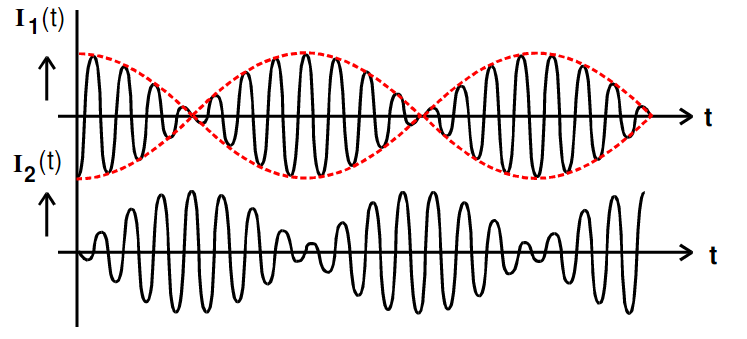
\includegraphics[scale=0.4]{schwebung.png}
  \caption{Amplitudenverlauf zweier Schwingungen, wenn eine Schwebung eintritt.}
  \label{fig:2}
\end{figure}
Diese Art der Schwingung, wie in Abbildung \ref{fig:2} zu sehen, nennt man Schwebung.
Die Frequenz $\nu_- - \, \nu_+$, mit der die Gesamtenergie des Systems zwischen
den Schwingkreisen oszilliert, wird als Schwebungsfrequenz bezeichnet.

\section{Durchführung}
\subsection{Versuchsaufbau}
\label{sec:versuchsaufbau}
\begin{figure}
  \centering
  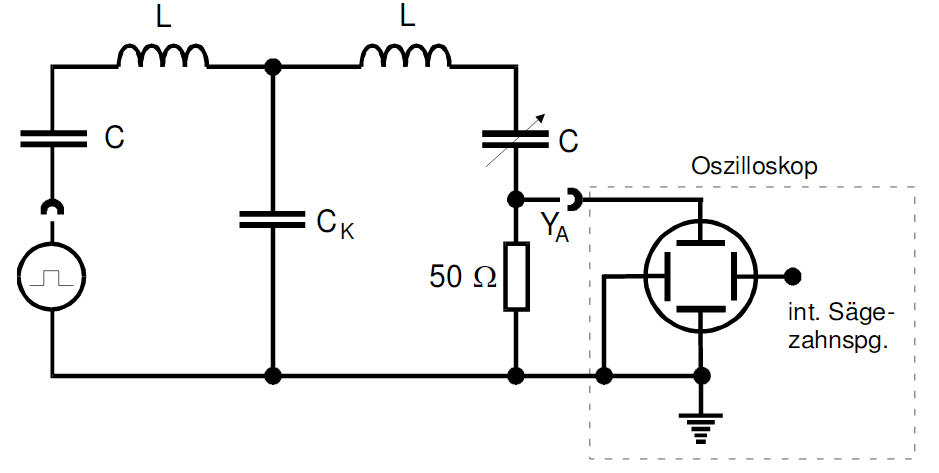
\includegraphics[scale=0.4]{aufbau.png}
  \caption{Schaltskizze zur Untersuchung des Schwebungsphänomens und,
  mit leichten Abwandlungen, zur Ermittlung der Fundamentalschwingungen.}
  \label{fig:3}
\end{figure}
Mit einer Rechteckspannung wird der linke $LC$ - Schwingkreis in Abbildung \ref{fig:3}
angeregt. Über den Kopplungskondensator $C_{\symup{K}}$ gelangt die Schwingung in den
rechten Teil des gekoppelten Schwingkreises (mit einem kapazitiv verstellbaren Kondensator),
wo über den einen ohmschen Widerstand ein Oszilloskop die Schwebung sichtbar macht.

Um die Fundamentalschwingungen zu bestimmen, wird in \ref{fig:3} die Rechteck- durch
eine Sinusspannung ersetzt und jene ebenfalls auf das Oszilloskop gegeben.

\subsection{Versuchsdurchführung}
\begin{figure}
  \centering
  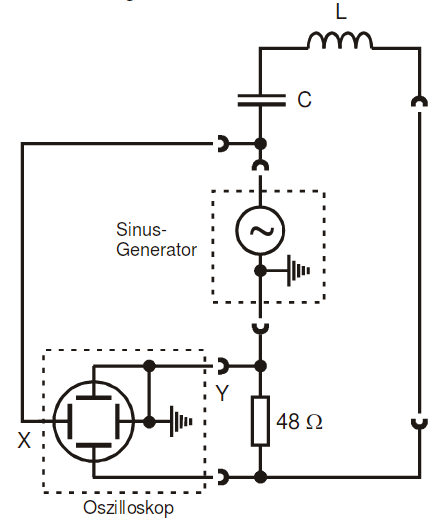
\includegraphics[scale=0.4]{justierung.png}
  \caption{Schaltskizze zur Justierung des einstellbaren Kondensators im rechten
  Schwingkreis in Abbildung \ref{fig:3}.}
  \label{fig:4}
\end{figure}
Zuerst wird mithilfe der Schaltung aus Abbildung \ref{fig:4} der rechte Schwingkreis unter Zuhilfenahme des einstellbare Kondensator
aus Kapitel \ref{sec:versuchsaufbau} auf die Resonanzfrequenz des anderen Schwingkreises eingestellt.
Zu diesem Zweck wird mit Hilfe von Lissajou-Figuren die Frequenz gesucht, bei der
die Phase zwischen Generatorspannung und Schwingkreisstrom im linken Schwingkreis gleich 0 ist.
Alsdann wird der Vorgang für den rechten Schwingkreis wiederholt, diesmal wird jedoch
die eben bestimmte Resonanzfrequenz durch den verstellbaren Kodensator eingestellt.

Um das Verhältnis zwischen Schwingungs- und Schwebungsfrequenz zu bestimmen, wird
für alle möglichen Kopplungskondensatoren $2 \le C_{\symup{K}} \le \SI{12}{\nano \farad}$
die Anzahl der Schwingungsmaxima innerhalb einer Schwebungsperiode gezählt. Dies
lässt sich über das Oszilloskop aus \ref{sec:versuchsaufbau} bewerkstelligen.

Weiterhin sollen die Fundamentalschwingungen $\nu_+$ und $\nu_-$ bestimmt werden.
Wie in Kapitel \ref{sec:versuchsaufbau} beschrieben werden Sinusspannung und Schwingkreisstrom
im Oszilloskop gegeneinander aufgetragen und mithilfe von Lissajou-Figuren die Frequenzen
gesucht, bei denen die Phase 0 ($\nu_+$, da $\nu_+ < \nu_-$) bzw. $\pi$ ($\nu_-$) ist.
Dabei werden erneut alle möglichen Kopplungskondensatoren $2 \le C_{\symup{K}} \le \SI{12}{\nano \farad}$
nacheinander eingeschaltet.

Eine andere Methode, um die Fundamentalschwingungen zu bestimmen, ist der sogennannte Sweep.
Dabei wird, in unserem Fall, in einer Sekunde das Frequenzspektrum von einer beliebigen
Anfangs- bis zu einer beliebigen Endfrequenz auf einem Oszilloskop dargestellt. Zu sehen
sind dann (neben zwei kleinen Peaks, die Anfangs- und Endzeitpunkt darstellen) zwei
große Peaks, die die Frequenzen $\nu_+$ und $\nu_-$ (in der Reihenfolge) darstellen.
Dies wird erneut in Abhängigkeit von $C_{\symup{K}}$ gemessen.

\section{Auswertung}

\section{Diskussion}
\newpage
\nocite{*}
\printbibliography
